\section{Faithful Generation}


\begin{frame}{Hallucination in Seq2Seq Models}


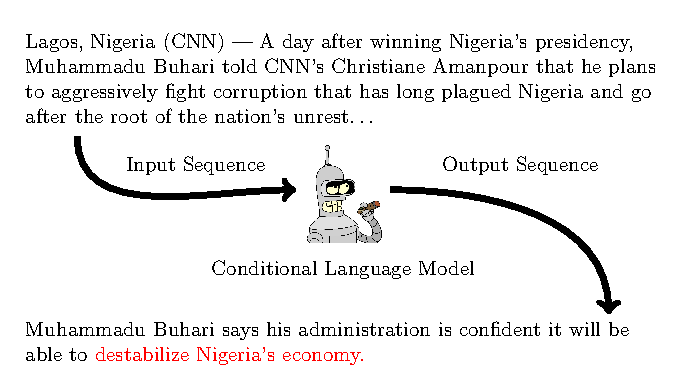
\includegraphics{4_fg/image_texs/clm/clm.pdf}


\end{frame}

\begin{frame}{Faithful Generation}



{\centering
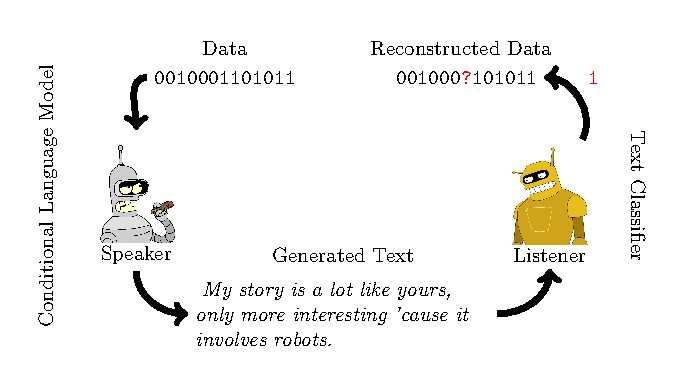
\includegraphics[scale=.7]{4_fg/image_texs/intro_pic/intro_pic.pdf}\\
}
%
\includegraphics[scale=.2]{images/section4/listener.jpeg}
%
\includegraphics[scale=.045]{images/section4/speaker.jpg}
\only<1>{ 
Inspired by:
\begin{itemize}
\item Rational Speakers and Listeners, (Andreas et al. )
\item $n$-best ranking,  (Collins and Koo)
\item Round-trip translation
\end{itemize}
}
\only<2>{
Motivation:
\begin{itemize}
\item Augment mle training with RL objective to improve accuracy of reconstruction without hurting fluency.
\item We can apply this object to entire beam search to encourage diverse but accurate generation outputs.
\item We can use the listener to give our confidence in the correctness of outputs.
\end{itemize}
}
\only<3>{
Other possible applications: controllable text generation.
}

\end{frame}

\begin{frame}{Two Applications}

    \begin{itemize}
        \item \textbf{Data-to-Text}
            \begin{itemize}
                \item Table data $\rightarrow$ text description $\rightarrow$ reconstruct table 
            \end{itemize} 
            ~\\~\\
        \item \textbf{Text-to-Text}
            \begin{itemize}
                \item Document text $\rightarrow$ text summary $\rightarrow$ answer cloze style questions from document
            \end{itemize}
    \end{itemize}

\end{frame}

\begin{frame}{Data-to-Text}
    \centering
    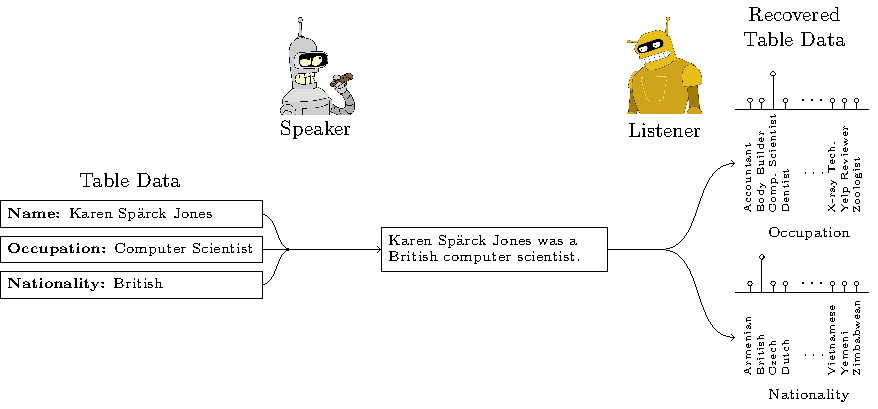
\includegraphics[scale=.8]{4_fg/image_texs/data2text/data2text.pdf}
\end{frame}
\begin{frame}{Text-to-Text}
    \centering
    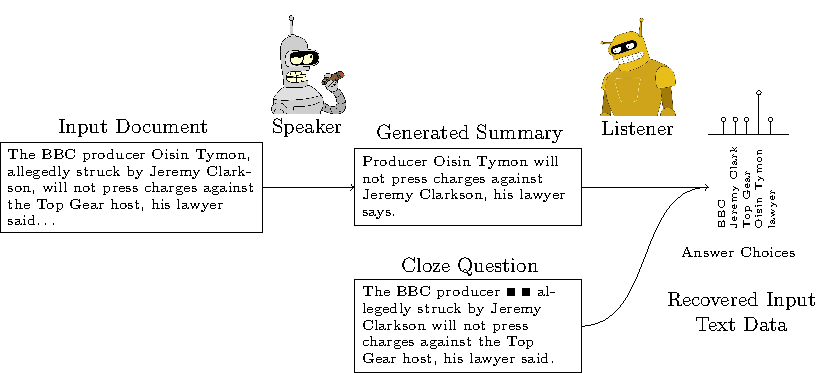
\includegraphics[scale=.8]{4_fg/image_texs/text2text/text2text.pdf}
\end{frame}



\begin{frame}{Planned Experiments}
    \begin{itemize}
            \only<1>{
        \item Data-to-Text
            \begin{itemize}
                \item E2E Dataset -- generate restaurant descriptions from metadata.
                \item WikiBio Datatest -- generate Wikipedia biographical entries from table data.
            \end{itemize}
        \item Text-to-Text
            \begin{itemize}
                \item TL;DR Dataset -- newly released, Reddit comments with 
                    summaries. (non-news dataset!)
                \item Lots of news (CNN/DM, NYT, Newsroom, XSUM)
            \end{itemize}
        }
        \only<2>{
        \item Reinforce (Williams ???) style learning objective to maximize
            correct classification by the listener.
        \item While incorrect statements in best beam candidate might be rare, errors more likely in remainder of beam.
        \item[$\Rightarrow$] Optimizing over whole beam should be easier to demonstrate 
            improvements.
        }
            \only<3>{
        \item Interesting angles to take even if performance improvements are not staggering:
            \begin{itemize}
                \item Apply listener as 
                    beam re-ranking criterion during generation.
                \item Understand correlation in listener models $\Rightarrow$ 
                    enforce independent listener models.
                \item Localize error signals with token level explanations 
                    from classifier.
               \end{itemize}
           }
           \only<4>{
           \item We can also focus on the cloze question generation aspect.
            \begin{itemize}
                \item Many heuristics for creating cloze style questions.
                \item Incorporate word importance model.
                \item Guided question generation to improve training.
            \end{itemize}

           }
    \end{itemize}
   
    

\end{frame}


